\documentclass[journal,a4paper]{IEEEtran}

\usepackage{amsmath,amssymb,amsfonts}
\usepackage{booktabs}
\usepackage{graphicx}
\usepackage{url}
\usepackage{xcolor}
\usepackage{algorithm}
\usepackage{algpseudocode}
\usepackage{multirow}
\usepackage[numbers,sort&compress]{natbib}
\usepackage{tikz}
\usetikzlibrary{arrows.meta,positioning,fit,backgrounds,calc}
\usepackage[hidelinks]{hyperref}

\graphicspath{{../results/figures/}}
\newcommand{\inputifexists}[1]{\IfFileExists{#1}{\input{#1}}{\textit{[table pending]}}}

\begin{document}

\title{CSLL: Complex Spectral Lead--Lag Networks for\\
Delay-Aware Multivariate Time-Series Forecasting}

\author{Francois Petizon\\[2pt]
{\normalsize Independent Researcher\ \ $\cdot$\ \ \href{mailto:francois.petizon9@icloud.com}{francois.petizon9@icloud.com}}}

\markboth{Preprint --- July 2025}{Petizon: Complex Spectral Lead--Lag Networks}

\maketitle

\begin{abstract}
Most multivariate forecasters that model dependencies \emph{between} series do so in a
\emph{phase-blind} way: cross-variate attention, channel-mixing MLPs, and spectral or graph
models represent inter-series coupling as real-valued and same-timestep, and cannot express that
one series \emph{leads} another by a delay. We ask a single question: \emph{when} does modelling
that lead--lag delay improve forecasts? We introduce a cross-channel operator applied per
frequency band whose \emph{phase} encodes a continuous inter-series delay (exact by the Fourier
shift theorem), factorised to $\mathcal{O}(N)$ via additive delays and gated onto a
channel-independent backbone. Two design choices make the mechanism testable rather than merely
plausible: a zero-padded transform, so the phase is a \emph{linear} (physical) shift rather than a
circular one, and a \emph{direct} synthesis of the shifted spectrum at the horizon, so the
forecast-optimal delay equals the physical delay. On planted-delay data the operator recovers the
true delays exactly (slope ${\approx}1$, $r{=}1.00$) where a naive estimator collapses.
Empirically we find a clear dichotomy: on data with delayed cross-series structure (weekly
regional influenza) the phase branch lowers a lightweight model's error by $13$--$19\%$ over
three seeds, closing most of the gap from a linear model to a cross-variate Transformer at an
order of magnitude fewer parameters; on same-time-dominated data (5-minute traffic, standard
long-horizon benchmarks) real-valued mixing suffices and the phase branch is redundant or mildly
harmful. Because simple a-priori statistics of the inter-series lead do \emph{not} cleanly predict
the regime, we introduce a gated \emph{hybrid} that runs a phase and a mixing branch and learns
their blend: one model that, without a regime label, stays within seed noise of the best
specialised variant everywhere and removes the same-time regression a phase-only model suffers. We
report where the mechanism helps, where it is redundant, and where a strong backbone subsumes it,
rather than a single headline number.
\end{abstract}

\begin{IEEEkeywords}
multivariate time series forecasting, cross-series dependence, frequency domain, lead--lag,
spectral methods, deep learning
\end{IEEEkeywords}

% ======================================================================
\section{Introduction}
\label{sec:intro}
Multivariate time-series forecasting (MTSF) predicts the joint future of $N$ interacting series
from shared history, underpinning traffic management, energy planning, and epidemiology. A central
design question is whether---and how---to model dependencies \emph{across} series.
Channel-independent (CI) models such as PatchTST~\citep{nie2023patchtst} and
DLinear~\citep{zeng2023dlinear} forecast each series separately and are strikingly hard to
beat~\citep{han2024capacity}; channel-dependent (CD) models such as
iTransformer~\citep{liu2024itransformer} and Crossformer~\citep{zhang2023crossformer} mix across
series for higher capacity. A recent line of critique~\citep{brigato2025champions,abdelmalak2025biased}
shows that on the standard benchmarks these rankings are fragile and the datasets are largely
self-predictable---which is exactly why CI models look so strong.

We focus on a specific, physically-motivated weakness shared by essentially all CD models: they
represent cross-series coupling as \emph{real-valued} and \emph{same-timestep}. iTransformer
attends over variate tokens at aligned times; channel-mixing MLPs mix instantaneously; spectral
and graph models learn real-valued spectral graphs or a frequency-shared complex transform that
encodes no phase. None can express that series $j$ \emph{leads} series $i$ by a delay---even though
propagation delays are physically ubiquitous (an upstream sensor leads a downstream one; an
epidemic reaches regions in sequence). The methods that target lead--lag, LIFT~\citep{zhao2024lift}
and VCformer~\citep{yang2024vcformer}, work in the time domain with discrete integer shifts; even
the one frequency-domain cross-channel operator we are aware of, Fredformer~\citep{piao2024fredformer},
mixes channels per band with real-valued attention and encodes no delay.

Rather than assert that a delay-aware operator is better, we ask \emph{when} it is. Our
contribution is a mechanism that makes the question answerable, an honest map of its answer, and a
model that acts on that map.

\paragraph{Contributions}
\begin{enumerate}
\item A complex spectral lead--lag operator (Sec.~\ref{sec:method}, Fig.~\ref{fig:arch}) with an
\emph{exact-delay} property, made physical and identifiable by a zero-padded linear-shift transform
and a head-free \emph{direct} forecast, so the forecast-optimal delay is the physical delay.
\item A correlation-initialised estimator that escapes the oscillatory time-delay-estimation loss
surface and recovers planted delays exactly, where a naive gradient-only estimator collapses
(Sec.~\ref{sec:killtest}, Fig.~\ref{fig:killtest}).
\item An empirical characterisation of \emph{when} phase-aware coupling helps---a clear dichotomy
between delayed-structure data (epidemics) and same-time data (traffic, standard benchmarks)---and
the honest negative result that simple a-priori lead statistics do not predict the split
(Sec.~\ref{sec:envelope}).
\item A gated \emph{hybrid} (Eq.~\ref{eq:hybrid}) that adapts across the dichotomy: without a
regime label it stays within seed noise of the best specialised variant in each regime, keeping the
epidemic gain while removing the same-time regression a phase-only model suffers
(Sec.~\ref{sec:results}). This, with its efficiency, is the practical model contribution.
\end{enumerate}

% ======================================================================
\section{Related Work}
\label{sec:related}
\paragraph{Classical and deep forecasters} Classical multivariate forecasting rests on vector
autoregression and the Box--Jenkins tradition~\citep{boxjenkins1970,luetkepohl2005}; VAR remains a
useful linear cross-series baseline. Deep long-horizon forecasting was reshaped by efficient
Transformers---Informer~\citep{zhou2021informer}, Autoformer~\citep{wu2021autoformer},
FEDformer~\citep{zhou2022fedformer}, Pyraformer~\citep{liu2022pyraformer}---and by decomposition
and basis-expansion models such as N-BEATS~\citep{oreshkin2020nbeats},
N-HiTS~\citep{challu2023nhits} and TimesNet~\citep{wu2023timesnet}. Autoformer's Auto-Correlation
aggregates \emph{within-series} periods, not inter-series lead--lag---a distinction central to our
work.

\paragraph{Channel strategies} DLinear/NLinear~\citep{zeng2023dlinear} and
PatchTST~\citep{nie2023patchtst} are channel-independent; iTransformer~\citep{liu2024itransformer},
Crossformer~\citep{zhang2023crossformer} and TSMixer~\citep{chen2023tsmixer} are channel-dependent,
with TiDE~\citep{das2023tide} and RLinear~\citep{li2023rlinear} as strong MLP/linear points on the
spectrum. \citet{han2024capacity} frame the CI/CD trade-off as capacity versus robustness under
distribution shift, and show it is not fundamental. Lightweight models push cost
down---SparseTSF~\citep{lin2024sparsetsf}, CycleNet~\citep{lin2024cyclenet},
SOFTS~\citep{han2024softs}---and channel clustering~\citep{chen2024ccm} interpolates CI and CD.
CSLL's gated additive branch is a spectral channel-partiality mechanism, and the hybrid makes the
CI$\leftrightarrow$CD position itself learnable per dataset.

\paragraph{Frequency-domain and cross-variate models} A large body of work forecasts in the
spectral domain. FEDformer~\citep{zhou2022fedformer} and FiLM~\citep{zhou2022film} operate on
selected frequency modes; FITS~\citep{xu2024fits} is a tiny complex-valued interpolator;
FilterNet~\citep{yi2024filternet} and FilterTS~\citep{wang2025filterts} learn frequency filters;
FreTS~\citep{yi2023frets} applies complex MLPs with weights shared across all bins and hence
carries no phase. Spatio-temporal graph models---Graph WaveNet~\citep{wu2019graphwavenet},
MTGNN~\citep{wu2020mtgnn}, StemGNN~\citep{cao2020stemgnn}---and FourierGNN~\citep{yi2023fouriergnn}
learn real-valued (spectral) graphs, and Fourier neural operators~\citep{li2021fno,guibas2022afno}
provide the general operator-learning backdrop. The closest to us,
Fredformer~\citep{piao2024fredformer} and FreEformer~\citep{yue2025freeformer}, mix channels
\emph{inside} the spectrum but with real-valued or data-driven attention, encoding no explicit,
interpretable delay; SimpleTM~\citep{chen2025simpletm} uses phase-sensitive wavelet tokens but not
as an inter-series delay. CSLL differs by making the phase of the cross-channel operator an
explicit, bounded, continuous delay with an additive $\mathcal{O}(N)$ factorisation.

\paragraph{Lead--lag and cross-variate delay} A small but growing line targets inter-series
lead--lag directly. LIFT~\citep{zhao2024lift} detects leading indicators by cross-correlation,
estimates an \emph{integer} leading step per channel at each time, and shifts the lagged variates
to align them---a time-domain add-on over a backbone. VCformer~\citep{yang2024vcformer} integrates
multi-step lagged cross-correlations inside the attention weights, again in the time domain, and
DeformTime~\citep{shu2025deformtime} learns dependencies across variables at different time steps
through deformable-attention offsets. All three are discrete, time-domain, and---by working through
learned shifts or attention---do not expose a continuous, bounded delay that can be read off and
checked against physics. Our operator instead places the lead--lag entirely in the \emph{phase} of
a per-band complex coupling: a single real number per channel pair, continuous (including
fractional delays), bounded to the identifiable range, and factorised additively so the cost stays
$\mathcal{O}(N)$. To our knowledge this specific combination---phase-as-continuous-delay with an
additive $\mathcal{O}(N)$ factorisation and a head-free direct forecast---is not present in prior
work.

\paragraph{Spatio-temporal and epidemic forecasting} Our evaluation uses datasets with known
geography: METR-LA/PEMS-BAY~\citep{li2018dcrnn} and PEMS04/08~\citep{guo2019astgcn} carry road
distances; the Cola-GNN regional influenza sets~\citep{deng2020colagnn} carry adjacency graphs. We
use these graphs only to \emph{validate} learned delays, not to train, so the comparison to graph
models~\citep{wu2019graphwavenet2} concerns interpretability, not leaderboard position.

\paragraph{Foundation models and evaluation} Pretrained forecasters~\citep{das2024timesfm,
ansari2024chronos,woo2024moirai,liu2025timerxl} are largely univariate-per-channel or use generic
attention for cross-series structure. Evaluation critiques~\citep{brigato2025champions,
abdelmalak2025biased} motivate our protocol: a uniform training budget, reported significance, and
datasets chosen for genuine cross-series structure.

% ======================================================================
\section{Method: CSLL and the Gated Hybrid}
\label{sec:method}
\paragraph{Intuition} Shifting a signal in time does not change how much of each frequency it
contains, only \emph{when} each frequency's oscillation peaks. That timing offset is a phase, and
it grows linearly with frequency at a rate equal to the delay---so one number per pair of series
captures the delay at every frequency at once. Modelling cross-series coupling as a per-band
complex weight whose \emph{magnitude} is the coupling strength and whose \emph{phase} is a
frequency-linear ramp therefore expresses ``series $i$ is a scaled, delayed copy of series $j$''
exactly and cheaply. The rest of this section makes that precise and addresses the two ways a naive
implementation breaks it (a circular rather than linear shift, and a projection head that hides the
delay).

\paragraph{Setup} Given a look-back $X\in\mathbb{R}^{N\times L}$ we predict
$\hat{Y}\in\mathbb{R}^{N\times H}$. We use a zero-padded real DFT of length $M=2L$, giving
$F=M/2+1$ bins at $\omega_f=2\pi f/M$; the padding makes the phase ramp a \emph{linear} shift.

\begin{figure*}[t]\centering
\resizebox{0.95\textwidth}{!}{%
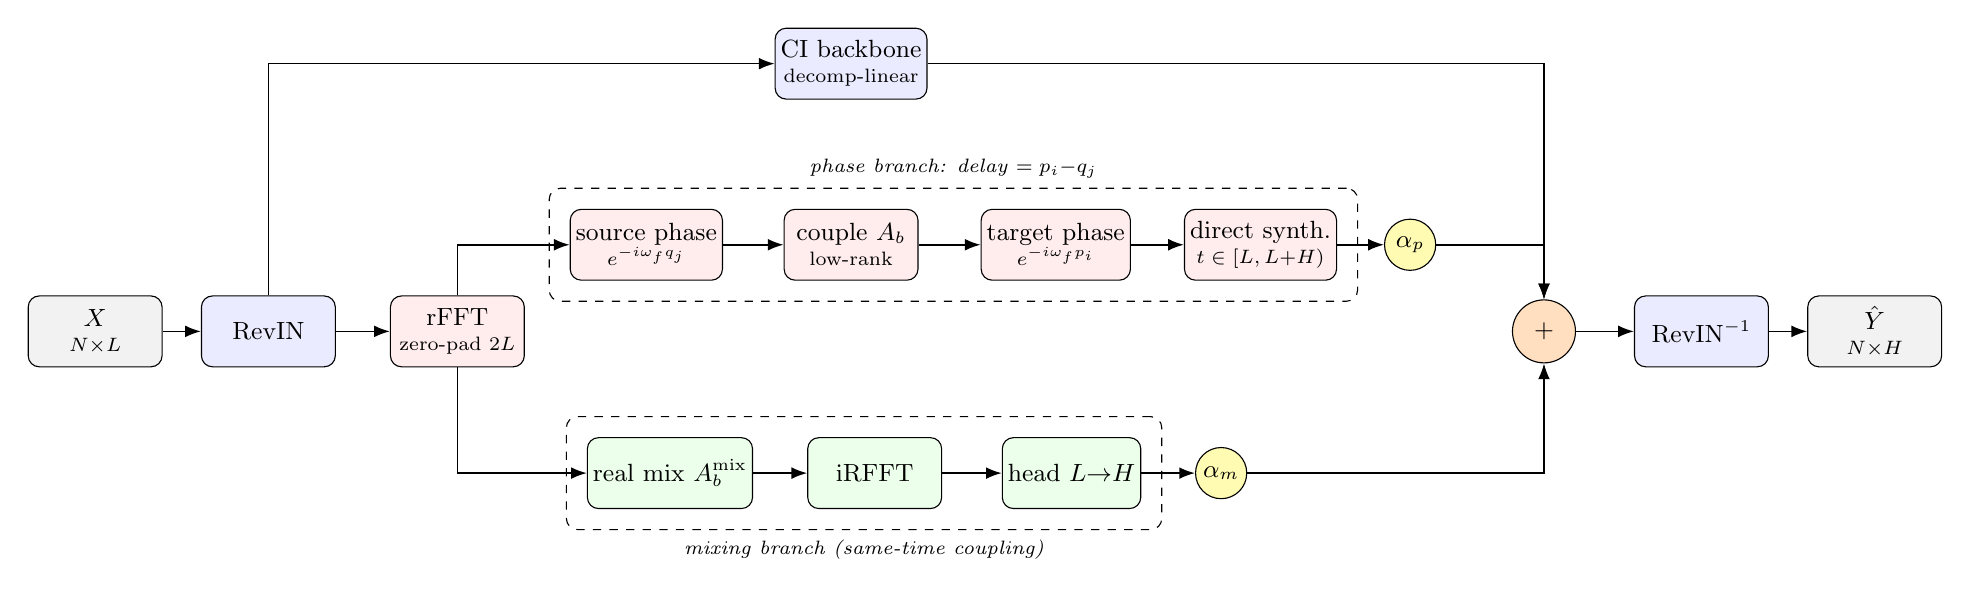
\begin{tikzpicture}[
  font=\small, >=Latex,
  box/.style={draw, rounded corners, minimum height=9mm, minimum width=17mm, align=center, inner sep=2pt},
  io/.style={box, fill=gray!10},
  bb/.style={box, fill=blue!8},
  ph/.style={box, fill=red!7},
  mx/.style={box, fill=green!8},
  g/.style={draw, circle, inner sep=0.5pt, minimum size=6.5mm, fill=yellow!30},
  sm/.style={draw, circle, inner sep=1pt, minimum size=8mm, fill=orange!25},
  arr/.style={-{Latex[length=2mm]}, semithick}]
  % --- spine ---
  \node[io] (x)     at (0,0)     {$X$\\[-2pt]{\scriptsize$N{\times}L$}};
  \node[bb] (revin) at (2.2,0)   {RevIN};
  \node[ph] (fft)   at (4.6,0)   {rFFT\\[-2pt]{\scriptsize zero-pad $2L$}};
  \node[bb] (back)  at (9.6,3.4) {CI backbone\\[-2pt]{\scriptsize decomp-linear}};
  % --- phase branch (top row, y=1.1) ---
  \node[ph] (sq)  at (7.0,1.1)  {source phase\\[-2pt]{\scriptsize$e^{-i\omega_f q_j}$}};
  \node[ph] (Aph) at (9.6,1.1)  {couple $A_b$\\[-2pt]{\scriptsize low-rank}};
  \node[ph] (sp)  at (12.2,1.1) {target phase\\[-2pt]{\scriptsize$e^{-i\omega_f p_i}$}};
  \node[ph] (dir) at (14.8,1.1) {direct synth.\\[-2pt]{\scriptsize$t\in[L,L{+}H)$}};
  \node[g]  (gph) at (16.7,1.1) {$\alpha_p$};
  % --- mixing branch (bottom row, y=-1.8) ---
  \node[mx] (Amx)  at (7.3,-1.8)  {real mix $A^{\mathrm{mix}}_b$};
  \node[mx] (imx)  at (9.9,-1.8)  {iRFFT};
  \node[mx] (head) at (12.4,-1.8) {head $L{\to}H$};
  \node[g]  (gmx)  at (14.3,-1.8) {$\alpha_m$};
  % --- merge (well clear to the right of both gates) ---
  \node[sm] (sum) at (18.4,0)   {$+$};
  \node[bb] (den) at (20.4,0)   {RevIN$^{-1}$};
  \node[io] (y)   at (22.6,0)   {$\hat Y$\\[-2pt]{\scriptsize$N{\times}H$}};
  \begin{scope}[on background layer]
    \node[draw, dashed, rounded corners, fit=(sq)(Aph)(sp)(dir), inner sep=2.6mm,
      label={[font=\scriptsize\itshape]above:phase branch: delay $=p_i{-}q_j$}] {};
    \node[draw, dashed, rounded corners, fit=(Amx)(imx)(head), inner sep=2.6mm,
      label={[font=\scriptsize\itshape]below:mixing branch (same-time coupling)}] {};
  \end{scope}
  \draw[arr] (x) -- (revin);
  \draw[arr] (revin) -- (fft);
  \draw[arr] (revin.north) |- (back.west);
  \draw[arr] (fft.north) |- (sq.west);
  \draw[arr] (fft.south) |- (Amx.west);
  \draw[arr] (sq) -- (Aph); \draw[arr] (Aph) -- (sp); \draw[arr] (sp) -- (dir); \draw[arr] (dir) -- (gph);
  \draw[arr] (Amx) -- (imx); \draw[arr] (imx) -- (head); \draw[arr] (head) -- (gmx);
  \draw[arr] (back.east) -| (sum.north);
  \draw[arr] (gph) -| (sum.north);
  \draw[arr] (gmx) -| (sum.south);
  \draw[arr] (sum) -- (den); \draw[arr] (den) -- (y);
\end{tikzpicture}}
\caption{CSLL hybrid architecture. A channel-independent backbone is corrected by two gated
spectral branches. The \emph{phase} branch applies a per-band complex operator whose phase encodes
a continuous inter-series delay $p_i{-}q_j$ and forecasts by synthesising the shifted spectrum
\emph{directly} at the future positions; a zero-delay band reads the zero padding and contributes
nothing, so it cannot express same-time coupling. The \emph{mixing} branch supplies that via
real-valued spectral coupling and an $L{\to}H$ head. Warm gates $\alpha_p,\alpha_m$ let the data
choose the blend, so one model spans delayed-structure and same-time regimes.}
\label{fig:arch}
\end{figure*}

\paragraph{Spectral lead--lag branch} With $\check X=\mathrm{rFFT}(\tilde X)$, for band $b$ and
bin $f\in\mathcal{B}_b$,
\begin{equation}\label{eq:op}
W_b(f)_{ij}=(A_b)_{ij}\,e^{-i\omega_f (D_b)_{ij}},\qquad (D_b)_{ij}=p_i-q_j,
\end{equation}
with $p_i,q_j=\tfrac{\tau_{\max}}{2}\tanh(\cdot)$ so $|(D_b)_{ij}|\le\tau_{\max}$ stays inside the
wrap-free identifiable range. The additive form factorises~\eqref{eq:op} into a per-channel source
phase, a coupling matmul ($A_b$ full, or low-rank $U_bV_b^\top$ for large $N$), and a per-channel
target phase---$\mathcal{O}(N)$ phase work. A small controller can make $p_i,q_i$ input-dependent
(the \emph{dynamic} variant).

\paragraph{Direct forecast} Rather than reconstruct the look-back and map it to the horizon with a
head, we synthesise the shifted spectrum directly at $t\in[L,L+H)$. With a head, the loss-optimal
delay for a pair with physical lag $\tau$ is $\tau-h$ (the head absorbs the horizon); the head-free
direct forecast makes the forecast-optimal delay equal $\tau$. Positions beyond the representable
lead ($h\ge\tau$) read the zero padding, and the gated backbone covers that residual.

\paragraph{Exact-delay property and identifiability} For a zero-padded signal the linear shift by
$\tau$ has DFT $e^{-i\omega_f\tau}\hat S(f)$ exactly (no wraparound), so if within a band series $i$
is a scaled delayed copy of $j$, one $(a,\tau)$ pair reproduces its contribution at every
frequency. A real mixer ($D_b\!\equiv\!0$) can only represent $\tau=0$. Sharing $(A_b,D_b)$ across a
band pins $|A_b|$ (flat magnitude) and $D_b$ (phase slope). The additive gauge
$(p,q)\!\to\!(p+c,q+c)$ leaves $D$ unchanged; we fix it by mean-centring the delay read-out.

\paragraph{Estimator} The MSE is oscillatory in $D$ (period set by the dominant signal period), so
gradient descent from $D=0$ finds the nearest local minimum---the classic time-delay-estimation
trap. We initialise $p,q$ from lagged cross-correlation (a two-pass global estimate, or a
weighted least-squares solve on the pairwise-lag graph for network data), then refine by gradient
training. Sec.~\ref{sec:killtest} shows this is necessary and sufficient for exact recovery.

\paragraph{Hybrid: one model across the dichotomy} Because the phase branch cannot express
same-time coupling, forcing all correction through it is harmful on same-time data. We run
\emph{both} a direct-phase branch and a real mixing branch (real spectral coupling, full-window
synthesis, then an $L{\to}H$ head), each behind its own warm gate (Fig.~\ref{fig:arch}):
\begin{equation}\label{eq:hybrid}
\hat{Y}=\hat{Y}^{\text{base}}+\alpha_{p}\,\hat{Y}^{\text{phase}}+\alpha_{m}\,\hat{Y}^{\text{mix}},
\ \text{then RevIN}^{-1}.
\end{equation}
Where the phase branch does not lower validation error its gate decays toward zero and mixing
carries the correction; where it does, the phase gate grows. The mixing branch adds only a low-rank
coupling and one head ($\mathcal{O}(Nr+LH)$ parameters).

\paragraph{Complexity} The per-band operator costs $\mathcal{O}(N^2F)$ dense, or
$\mathcal{O}(NrF)$ with the rank-$r$ coupling; the additive delays contribute $\mathcal{O}(N)$
phase work per bin rather than a per-bin $N{\times}N$ operator. With the real-arithmetic
(cos/sin) DFT the whole model is real matmuls and is device-agnostic. The operator adds
$B(2Nr+2N)$ parameters---a few tens of thousands for the datasets here---against the
hundreds of thousands of a cross-variate Transformer, and trains several times faster
(Sec.~\ref{sec:results}). Delays are bounded by $\tau_{\max}=L/2$, so the representable lead scales
with the look-back.

\begin{algorithm}[t]
\caption{CSLL hybrid forward pass}\label{alg:csll}
\begin{algorithmic}[1]
\State $\tilde X\gets\mathrm{RevIN}(X)$;\ \ $\hat Y^{\text{base}}\gets\mathrm{DecompLinear}(\tilde X)$
\State $(\check X_r,\check X_i)\gets\mathrm{rFFT}_{2L}(\tilde X)$
\For{band $b$, bins $f\in\mathcal{B}_b$} \Comment{phase branch}
  \State apply source phase $e^{-i\omega_f q}$, couple $A_b$, target phase $e^{-i\omega_f p}$
\EndFor
\State $\hat Y^{\text{phase}}\gets\mathrm{Re}\,\mathrm{iDFT}_{t\in[L,L+H)}(\check Z)$ \Comment{direct}
\State $\hat Y^{\text{mix}}\gets\mathrm{head}(\mathrm{iRFFT}(A^{\text{mix}}\check X))$
\State \Return $\mathrm{RevIN}^{-1}(\hat Y^{\text{base}}+\alpha_p\hat Y^{\text{phase}}+\alpha_m\hat Y^{\text{mix}})$
\end{algorithmic}
\end{algorithm}

% ======================================================================
\section{Does the Estimator Recover Delays?}
\label{sec:killtest}
We construct a leader--follower regime: a white-noise leader drives followers that are pure
delayed copies with planted lags $\tau_i$, so each follower is forecastable \emph{only} through the
correctly delayed cross-series link. Table~\ref{tab:killtest} and Fig.~\ref{fig:killtest} report
test MSE and delay recovery. The naive estimator (no correlation init, circular shift, cold gate)
fails---MSE far above the information floor, recovery slope ${\approx}0$. The full estimator reaches
the floor with exact recovery (slope ${\approx}1$, $r=1.00$), and each fix is individually
necessary (removing the correlation init alone reverts recovery to ${\approx}0$). This isolates
estimation from the downstream question of whether real data \emph{has} recoverable delays.

\begin{table}[t]\centering\small
\caption{Kill-test (leader--follower, planted delays): the v2 estimator recovers delays exactly;
ablating any fix breaks it.}
\label{tab:killtest}
\resizebox{\columnwidth}{!}{%
\begin{tabular}{lccc}
\toprule
Estimator & test MSE & rec.\ slope & $r$ \\
\midrule
naive (cold gate, circular) & 0.527 & $-0.02$ & $-0.18$ \\
\ + fixes, no corr.\ init & 0.879 & 0.02 & 0.36 \\
\textbf{full estimator} & \textbf{0.154} & \textbf{0.99} & \textbf{1.00} \\
\midrule
information floor & ${\approx}0.147$ & --- & --- \\
\bottomrule
\end{tabular}}
\end{table}

\begin{figure}[t]\centering
\IfFileExists{../results/figures/fig_killtest.pdf}{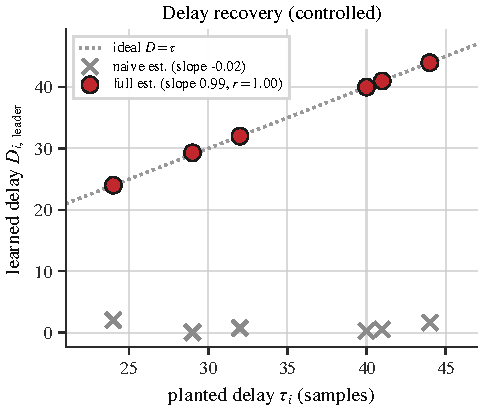
\includegraphics[width=0.72\columnwidth]{fig_killtest.pdf}}{\fbox{[fig\_killtest pending]}}
\caption{Controlled delay recovery: the full estimator (red) lands on the identity; the naive
estimator (grey) collapses to near-zero.}
\label{fig:killtest}
\end{figure}

% ======================================================================
\section{When Does Phase Help? An Empirical Dichotomy}
\label{sec:envelope}
\paragraph{The dichotomy} We measure the phase branch's value directly as the relative test-MSE
change from a real-valued mixer to the phase operator, holding everything else fixed
(Table~\ref{tab:envelope}). The split is clean by \emph{data}, not model: on all three regional
influenza datasets the phase branch helps substantially ($+13$--$19\%$), while on 5-minute traffic
and the standard benchmarks it is neutral-to-harmful (up to a $17\%$ regression on Weather).
Influenza carries delayed cross-region structure---an epidemic reaches regions in sequence over
weeks---that a same-time mixer cannot represent but a complex, phase-carrying operator can; traffic
and the benchmark series are dominated by same-time coupling, where the extra phase capacity only
adds variance.

\paragraph{An honest negative: lead statistics do not predict the split} It is tempting to seek a
cheap a-priori statistic that says which regime a dataset is in. We tried two. A lead/horizon
ratio $\bar\tau/H$ (mean cross-correlation lag over coupled pairs) over-predicts a phase benefit on
traffic. A \emph{delay advantage} $\Delta(H)=\mathbb{E}_i[\rho_{\ge H}(i)-\rho_0(i)]$---whether a
partner leading by at least $H$ predicts series $i$ better than any same-time partner---correctly
marks traffic as a mixing regime ($\Delta\ll0$) but also comes out negative on most influenza
settings, where the phase nonetheless helps (the benefit there is the added expressiveness of
complex over real mixing, not a single dominant leading partner). Across our settings
$\mathrm{sign}\,\Delta(H)$ agrees with the outcome in fewer than half of settings
(Table~\ref{tab:envelope}, Fig.~\ref{fig:envelope}). We therefore do \emph{not} offer a predictive
scalar; we take the practical route (Sec.~\ref{sec:results}): a hybrid that learns the blend per
dataset, removing the need to predict the regime.

\begin{table}[t]\centering\small
\caption{When phase beats mixing: measured phase-vs-mixing gain per setting. The split is clean by
data, but the a-priori statistic $\Delta(H)$ predicts it in fewer than half of settings (see footnote).}
\label{tab:envelope}
\resizebox{\columnwidth}{!}{\inputifexists{../results/tables/v2_envelope.tex}}
\end{table}

\begin{figure}[t]\centering
\IfFileExists{../results/figures/fig_envelope.pdf}{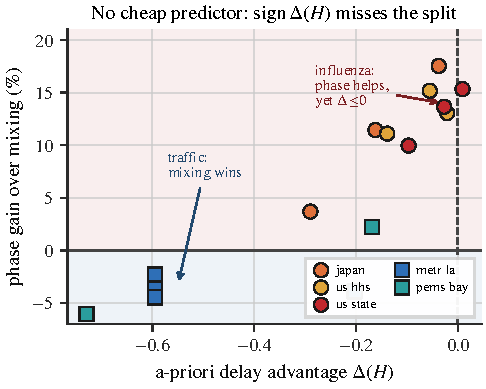
\includegraphics[width=0.98\columnwidth]{fig_envelope.pdf}}{\fbox{[fig\_envelope pending]}}
\caption{No cheap predictor: influenza (phase helps, top) sits at $\Delta\!\approx\!0$ while
traffic (mixing, bottom) sits at $\Delta\!\ll\!0$; the sign of $\Delta$ misses the split.}
\label{fig:envelope}
\end{figure}

% ======================================================================
\section{Experimental Setup}
\label{sec:setup}
\paragraph{Datasets} We evaluate on twelve public datasets in three families
(Table~\ref{tab:datasets}). Two carry \emph{ground-truth geography} that we use to validate
learned delays: 5-minute freeway traffic (METR-LA, PEMS-BAY~\citep{li2018dcrnn}, with sensor
road-distance graphs) and weekly regional influenza (US-state, Japan-prefecture, US-region, with
adjacency graphs~\citep{deng2020colagnn}). The standard long-term forecasting (LTSF) suite
(ETT$\times$4, Weather, Exchange, ILI) is a secondary control on which cross-series structure is
weak. The graphs are used only for post-hoc validation, never for training.

\begin{table}[t]\centering\small
\caption{Datasets. $N$: number of series; horizons in native sampling units.}
\label{tab:datasets}
\resizebox{\columnwidth}{!}{\inputifexists{../results/tables/v2_datasets.tex}}
\end{table}

\paragraph{Protocol} One shared harness: chronological splits; standardisation with train-only
statistics; RevIN~\citep{kim2022revin} for neural models; a \emph{uniform} training budget (30
epochs, early stopping, patience 5) for every model on the traffic and influenza data; MSE loss;
Adam. The gate is trained honestly---no post-hoc validation selection of the branch. Look-back
$L{=}96$ ($36$ for the short weekly series). METR-LA runs the full protocol (3 seeds, all
horizons); PEMS-BAY runs a disclosed reduced protocol (1 seed, $H\in\{12,96\}$) as the confirmation
speed benchmark. On the LTSF suite we use the 10-epoch budget standard in that literature so our
numbers are comparable to published baselines. We report MSE/MAE on standardised series and
Diebold--Mariano tests~\citep{diebold1995comparing} against the best baseline per setting. All runs
are CPU-only for reproducibility.

\paragraph{Baselines and configuration} We compare against SeasonalNaive, VAR (where tractable),
NLinear, DLinear, PatchTST and iTransformer, all in the shared harness, plus four internal
variants that isolate the mechanism: \emph{CI-backbone} (branch off), \emph{phase-off} (real
mixing, $D{\equiv}0$), \emph{static} (fixed delays), and the full dynamic model.
Table~\ref{tab:hp} lists the per-model configuration; CSLL uses 4 frequency bands,
$\tau_{\max}{=}L/2$, and a rank-16 coupling on the high-dimensional datasets.

\begin{table}[t]\centering\small
\caption{Model configuration (fixed across datasets; equal training budget).}
\label{tab:hp}
\begin{tabular}{@{}l p{0.62\columnwidth}@{}}
\toprule
Model & Configuration \\
\midrule
DLinear/NLinear & moving-avg kernel 25 (DLinear); lr $10^{-3}$ \\
PatchTST & patch 16 / stride 8, $d_{\text{model}}{=}64$, 2 layers, 4 heads; lr $3{\times}10^{-4}$ \\
iTransformer & $d_{\text{model}}{=}128$, 3 layers, 8 heads, FFN 256; lr $3{\times}10^{-4}$ \\
VAR & lag order by BIC ($\le 8$); low-$N$ datasets only \\
\textbf{CSLL} & 4 bands, $\tau_{\max}{=}L/2$, rank-16 coupling if $N{>}64$, dynamic delays,
xcorr init, warm gate $0.05$; lr $10^{-3}$ \\
\textbf{CSLL2H} & CSLL $+$ gated real-mixing branch (Eq.~\ref{eq:hybrid}) \\
\bottomrule
\end{tabular}
\end{table}

% ======================================================================
\section{Results}
\label{sec:results}

\paragraph{Phase-essential regime: regional influenza} On all three influenza datasets the phase
branch robustly improves the lightweight (linear-backbone) model over its real-mixing counterpart
(US-state $+15\%$, $0.354\!\to\!0.300$ at $H{=}2$; US-region $+13\%$; Japan $+17\%$; three seeds,
gap $\gg$ seed noise; Table~\ref{tab:epi}), closing most of the distance from the linear baselines
to the cross-variate Transformers at ${\sim}14\times$ fewer parameters. \emph{We do not claim
SOTA}: iTransformer and PatchTST win outright here (US-state $H{=}2$: iTransformer $0.252$, PatchTST
$0.265$, CSLL $0.300$), because a strong attention backbone already captures the cross-series
structure the phase branch supplies to a weak one (Sec.~\ref{sec:discussion}).

\begin{table*}[t]\centering\small
\caption{Regional influenza, test MSE (lower better). CSLL beats the linear baselines and its own
real-mixing variant; the strong Transformers remain best in absolute terms.}
\label{tab:epi}
\resizebox{0.92\textwidth}{!}{\inputifexists{../results/tables/v2_epi_mse.tex}}
\end{table*}

\paragraph{Sub-horizon regime: traffic} On 5-minute traffic, propagation is sub-horizon, so
real-valued mixing captures the dominant same-time congestion structure and the phase adds little.
On METR-LA the cheap spectral branch is competitive: it matches or beats DLinear, PatchTST and
iTransformer at a fraction of their parameters (Table~\ref{tab:st}, Fig.~\ref{fig:pareto}). On the
denser PEMS-BAY the cross-variate iTransformer is strongest and CSLL trails it (significantly at
$H{=}96$ by a Diebold--Mariano test); what \emph{does} carry over is the phase-versus-mixing
pattern---the phase branch does not improve on real mixing there either---so PEMS-BAY confirms the
same \emph{regime}, not a CSLL accuracy win.

\begin{table*}[t]\centering\small
\caption{Spatio-temporal traffic, test MSE. On METR-LA the cheap spectral model is competitive
with far larger baselines; on the denser PEMS-BAY (reduced protocol) iTransformer is strongest,
while the phase-versus-mixing pattern is unchanged.}
\label{tab:st}
\resizebox{0.92\textwidth}{!}{\inputifexists{../results/tables/v2_st_mse.tex}}
\end{table*}

\paragraph{One model across the dichotomy: the hybrid} Pure direct-phase, unable to express
same-time coupling, regresses where mixing is what helps---most sharply on the standard benchmarks
(Weather/$96$: phase-only $0.184$ vs.\ mixing $0.156$, a $17\%$ regression) and mildly on traffic.
The gated hybrid removes this: on Weather/$96$ it recovers $0.160$ (matching the mixing specialist),
on traffic it matches the mixing branch within ${\sim}1\%$, and on the phase-essential influenza it
keeps the phase gain (Table~\ref{tab:hybrid}). One model, without a regime label, is within seed
noise of the best specialised variant everywhere.

\begin{table}[t]\centering\small
\caption{The hybrid matches the best specialised branch in each regime with one model
(\textbf{bold} $=$ within $2\%$ of the best specialist).}
\label{tab:hybrid}
\resizebox{\columnwidth}{!}{\inputifexists{../results/tables/v2_hybrid.tex}}
\end{table}

\paragraph{Horizon behaviour} Fig.~\ref{fig:mseh} plots MSE against horizon in both regimes. On
influenza the full model (and its hybrid) tracks the strong baselines while its real-mixing
variant lags at every horizon; on traffic the ordering collapses---mixing and phase coincide and
all cheap models cluster below the Transformers.

\begin{figure}[t]\centering
\IfFileExists{../results/figures/fig_mseh.pdf}{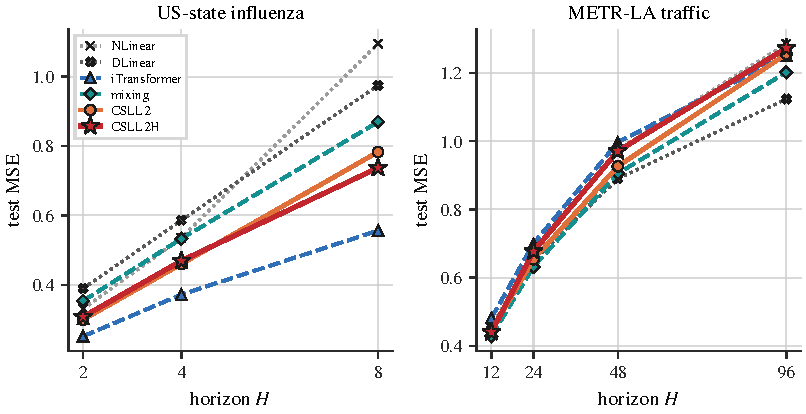
\includegraphics[width=\columnwidth]{fig_mseh.pdf}}{\fbox{[fig\_mseh pending]}}
\caption{MSE versus horizon. Left: US-state influenza (phase-essential)---the phase branch
separates from real mixing at every horizon. Right: METR-LA traffic (mixing)---phase and mixing
coincide; cheap spectral models sit below the Transformers.}
\label{fig:mseh}
\end{figure}

\paragraph{Ablation: isolating the components} Table~\ref{tab:ablation} adds the components one at
a time over a channel-independent backbone. On influenza, adding real mixing gives little, but
adding the \emph{phase} (static or dynamic) delivers the branch gain; on traffic and Weather the
mixing already captures the coupling and the phase adds nothing. The dynamic (input-adaptive)
delay is at best marginal over the static one---we report it as neutral rather than a contribution.

\begin{table}[t]\centering\small
\caption{Ablation (mean test MSE over horizons): components added over the CI backbone. The
\emph{branch gain vs CI} is the full model's improvement over the backbone.}
\label{tab:ablation}
\resizebox{\columnwidth}{!}{\inputifexists{../results/tables/v2_ablation.tex}}
\end{table}

\paragraph{LTSF control} On the standard benchmarks (Table~\ref{tab:ltsf}), where cross-series
structure is weak, CSLL behaves as a competent CI model: within $5\%$ of the best baseline in half
the settings and never far off, i.e.\ correctly near-inert. The one visible failure is exactly the
phase-hurts-mixing effect---on Weather the phase model ($0.184$ at $H{=}96$) trails its mixing
variant ($0.156$), and the hybrid ($0.162$) recovers most of the gap---which is why the LTSF
suite motivates, rather than contradicts, the hybrid.

\begin{table*}[t]\centering\small
\caption{Standard LTSF benchmarks, test MSE (10-epoch protocol, comparable to the literature).
CSLL is a competent channel-independent model here; the hybrid removes the phase regression
(e.g.\ Weather).}
\label{tab:ltsf}
\resizebox{0.92\textwidth}{!}{\inputifexists{../results/tables/v2_ltsf_mse.tex}}
\end{table*}

\paragraph{Efficiency and significance} CSLL uses tens of thousands of parameters against hundreds
of thousands for the Transformers and trains several times faster (Table~\ref{tab:eff},
Fig.~\ref{fig:pareto}). Diebold--Mariano tests against the best baseline per setting
(Table~\ref{tab:dm}) accompany the point estimates.

\begin{table}[t]\centering\small
\caption{Parameter count and mean training time (tractable datasets).}
\label{tab:eff}
\inputifexists{../results/tables/v2_efficiency.tex}
\end{table}

\begin{figure}[t]\centering
\IfFileExists{../results/figures/fig_pareto_v2.pdf}{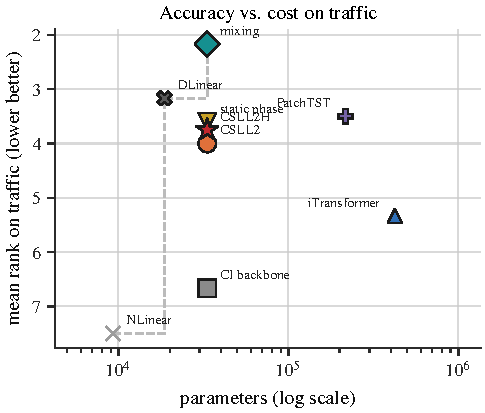
\includegraphics[width=0.98\columnwidth]{fig_pareto_v2.pdf}}{\fbox{[fig\_pareto pending]}}
\caption{Accuracy (average rank on traffic) versus parameters. CSLL variants ($\star$) sit at the
low-parameter end of the frontier.}
\label{fig:pareto}
\end{figure}

\begin{table}[t]\centering\small
\caption{Diebold--Mariano tests, CSLL vs.\ best baseline per setting
($\succ$/$\approx$/$\prec$: CSLL significantly better / tied / worse).}
\label{tab:dm}
\resizebox{\columnwidth}{!}{\inputifexists{../results/tables/v2_dm.tex}}
\end{table}

\paragraph{Interpretability: exact on controlled, partial on real} On planted-delay data the
operator recovers delays exactly (Sec.~\ref{sec:killtest}). The real datasets carry the structure:
a direct cross-correlation analysis of METR-LA recovers congestion back-propagation at
${\approx}16$\,km/h, inside the textbook 15--20\,km/h kinematic-wave range. The model's learned
delays, however, align with observed geography only weakly (Fig.~\ref{fig:delayreal}): on METR-LA
the learned-delay/road-distance relationship is noisy, and on influenza the input-conditioned
delays sit at the epidemiologically plausible multi-week scale but concentrate on the
border-adjacency graph only slightly. We read this as a limit of the ground truth (road distance
and shared borders are imperfect proxies for the effective coupling) as much as the model, and
claim \emph{plausible but not clean} delays on real data.

\begin{figure}[t]\centering
\IfFileExists{../results/figures/fig_delay_real.pdf}{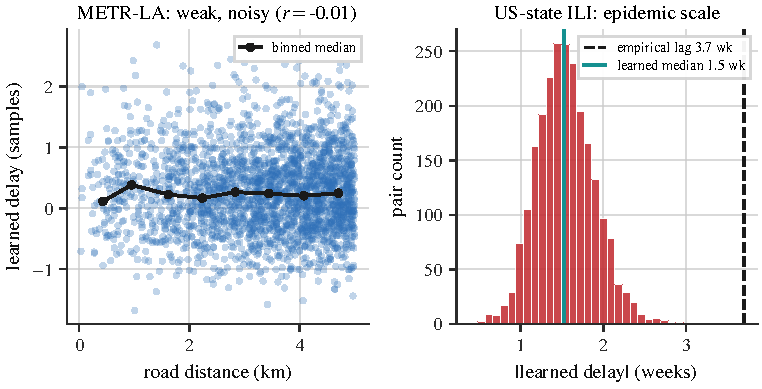
\includegraphics[width=0.98\columnwidth]{fig_delay_real.pdf}}{\fbox{[fig\_delayreal pending]}}
\caption{Learned delays on real data. Left: METR-LA learned delay vs.\ road distance (noisy).
Right: US-state ILI input-conditioned delay magnitudes at the epidemiologically plausible scale
(dashed: empirical inter-region lag).}
\label{fig:delayreal}
\end{figure}

% ======================================================================
\section{Discussion and Limitations}
\label{sec:discussion}
The dichotomy gives a design rule of thumb: phase/delay structure helps on data with delayed
cross-series coupling (epidemics, long-range propagation) and not on same-time-dominated data;
since simple statistics do not reliably tell the two apart in advance, the gated hybrid applies the
rule automatically by learning the blend. A second finding sets the scope of the mechanism's
\emph{value}: a strong cross-variate backbone \emph{subsumes} it. The phase branch improves a
lightweight CI backbone by $13$--$19\%$ on epidemic data, but grafting it onto an iTransformer
backbone yields no gain---the attention layers already capture the delayed structure the explicit
operator supplies to a weak backbone. Phase-as-delay is thus most valuable where capacity is
scarce: a cheap way to give a small model the cross-series reach of a large one.

\textbf{Limitations, stated plainly.}
(i) CSLL does not beat the strongest baselines in absolute accuracy; its case is efficiency,
adaptivity, and a characterised mechanism.
(ii) We do not provide an a-priori predictor of the regime: the lead statistics we tried fail
(Sec.~\ref{sec:envelope}); a reliable cheap predictor remains open.
(iii) Interpretability transfers imperfectly to real data (Sec.~\ref{sec:results}).
(iv) The dynamic delay variant helps little; we report it as neutral.
(v) The rFFT assumes within-window quasi-stationarity and bounds delays by $\tau_{\max}$.
(vi) PEMS-BAY uses a disclosed reduced protocol (1 seed, $H\in\{12,96\}$); we do not claim
per-setting significance there, only the qualitative regime. We do not benchmark against pretrained
foundation models, whose corpora may overlap our test data.

\paragraph{Future work} Three directions follow directly. First, a reliable a-priori regime
predictor: our lead statistics fail, but a small validation probe (train both branches briefly and
read the gates) may substitute cheaply for a closed-form statistic. Second, multi-modal delays: the
current operator favours a dominant lead per pair, whereas epidemics and transport networks carry a
\emph{distribution} of lags; a mixture of delay components per band is a natural extension. Third,
delay-aware pretraining: because the operator is cheap and interpretable, it could serve as a
structured, low-parameter cross-series head on top of a frozen univariate foundation model,
combining the reach of pretraining with an explicit, auditable coupling.

\paragraph{Broader impact} The datasets we study---traffic and epidemics---are decision-relevant,
and an interpretable delay matrix is attractive for operators who must justify forecasts. We
caution against the converse: the learned delays are predictive alignments, not causal claims, and
Sec.~\ref{sec:results} shows they align only weakly with physical geography on real data. Reading
them as causal transmission paths would be a misuse.

% ======================================================================
\section{Conclusion}
\label{sec:conclusion}
We turned a physical prior---that inter-series coupling carries frequency-dependent propagation
delays---into an exact, identifiable, cheap operator, and used it to answer \emph{when} phase-aware
cross-series modelling pays. The mechanism recovers planted delays exactly, helps a lightweight
model on genuinely lagged data (regional epidemics), and is redundant on same-time data; because no
cheap statistic predicts which regime holds, a gated hybrid learns the blend and is safe and
near-best across regimes with one model. We report where the mechanism helps, where it is
redundant, and where a strong backbone subsumes it, rather than a single headline number.

\section*{Reproducibility}
All datasets are public with fetch scripts and checksums; code, configs, fixed seeds, and scripts
to regenerate every table and figure accompany the paper.

\bibliographystyle{IEEEtranN}
\bibliography{references}

\end{document}
